\chapter{Referencial Teórico}

\section{Aprendizado Ativo}
Método pedagógico que envolve os estudantes no aprendizado, de maneira bastante simples
essa é a definição de aprendizado ativo. Em resumo, aprendizado ativo é qualquer coisa
que além de envolver os estudantes no fazer, os faça pensar no que estão fazendo \cite[p. 19]{Charles1991}.

Os princípios do aprendizado ativo são dois: introduzir atividades nas salas de aula
tradicionais e promover o envolvimento dos estudantes. O primeiro é a forma
mais simples do aprendizado ativo. Um exemplo seria fazer pequenas pausas na aula
e colocar os estudantes para revisar as notas de aula com um colega. No entanto,
é preciso que tais atividades promovam o engajamento dos estudantes no processo
de ensino e aprendizagem \cite[p. 3]{Prince2004}. Métodos ativos como Instrução
pelos Colegas \cite{} ...\footnote{colocar outros métodos ativos e resultados}

Em salas de aula que utilizam o aprendizado ativo pode-se ter um aumento de até 6\%
na média final nas provas dos alunos e que aquelas salas de aula puramente expositivas
têm 55\% mais chance de reprovarem os alunos do que aquelas com aprendizado ativo.
Esse aumento que pode parecer pouco (0,3 no GPA) colocaria a média daqueles estudantes
que desistem do curso bem próximo daqueles que permanecem, podendo-se dessa forma aumentar
a taxa de retenção dos estudantes \cite[p. 4]{Freeman2014}.

O estudo de meta-análise de \citeonline{Freeman2014} envolveu mais de 200 artigos
que comparavam as performances dos alunos em salas de aula com pelo menos algum
elemento de aprendizado ativo com as tradicionais aulas expositivas. Além de
mostrarem evidências de que o aprendizado ativo pode melhorar o aprendizado dos
estudantes de graduação principalmente nas áreas de ciência, tecnologia, engenharia
e matemática, \citeauthoronline{Freeman2014} propõem aos futuros pesquisadores
testarem não mais a eficiência dos métodos de aprendizado ativo frente as tradicionais
aulas expositivas (``primeira geração de pesquisas''), mas sim de verificar qual
o tipo de aprendizado ativo é mais apropriado para cada área do conhecimento
(``segunda geração de pesquisas'').

No entanto, tornar o aluno um agente ativo no processo de ensino e aprendizagem dado a realidade brasileira
não é uma tarefa fácil. Muitas são as adversidades de infraestrutura e institucionais
encontradas de modo a propiciar uma aprendizagem significativa. Seja por salas com
numero excessivo de alunos, estes desinteressados, professores mal pagos, ou com
a pressão de produzir cientificamente \cite{Araujo2013}.

Por outro lado, muitas são as iniciativas encontradas na literatura mostrando resultados
satisfatórios que podem ajudar o professor nesse processo \cite{Crouch2001, Gok2013, Barros2004}.
Na próxima seção será apresentado o método ativo de ensino \textit{Peer Instruction} ou \textit{Instrução pelos Colegas}
(IpC)\nomenclature{IpC}{Instrução pelos Colegas}.

\subsection{Instrução pelos Colegas (IpC)}
\label{section:ipc}

O IpC foi desenvolvido pelo Professor Eriz Mazur da Universidade de Harvard (EUA) na
década de 90. O objetivo do IpC é fazer com que todos os estudantes se engajem em
discussões com o vizinho de opinião diferente sobre um determinado conceito e fazer com que cada
estudante tente explicar o conceito um para o outro \cite{Mazur2009}.

No método IpC geralmente o professor começa fazendo uma breve exposição dialogada do conteúdo (15min).
Depois é colocado para os estudantes uma questão conceitual, que é
desenvolvida de modo a avaliar o entendimento dos estudantes sobre um tópico. Um
exemplo de uma questão conceitual de introdução a física é mostrada na \autoref{fig:desenv_ct}. Os
estudantes então individualmente respondem a questão (1-2min) geralmente utilizando
\textit{clickers}, que são pequenos dispositivos transmissores como os da \autoref{fig:desenv_clickers}.

Em seguida, dependendo do percentual de alunos que acertem a questão,
o professor pode revisar o assunto (acerto < 30\%), fazer uma breve explanação da
questão e ir para um próximo tópico ou nova questão (acerto > 70\%), ou o que se
deseja do método, um percentual de acerto entre 30\% e 70\% em que nessa situação o
professor estimula que os alunos encontrem um parceiro que respondeu preferencialmente de forma diferente
e que tentem explicar um para o outro o porquê de estar correto, ou seja, os alunos se auto
instruem temos então o nome do método ``Instrução pelos Colegas'' \cite{Mazur2009, Crouch2001}.
A \autoref{fig:desen_fluxograma_ipc} resume o processo de implementação do método IpC na sala de aula.

\begin{figure}[!htb]
  \centering
  \caption{Exemplo de uma questão conceitual}
  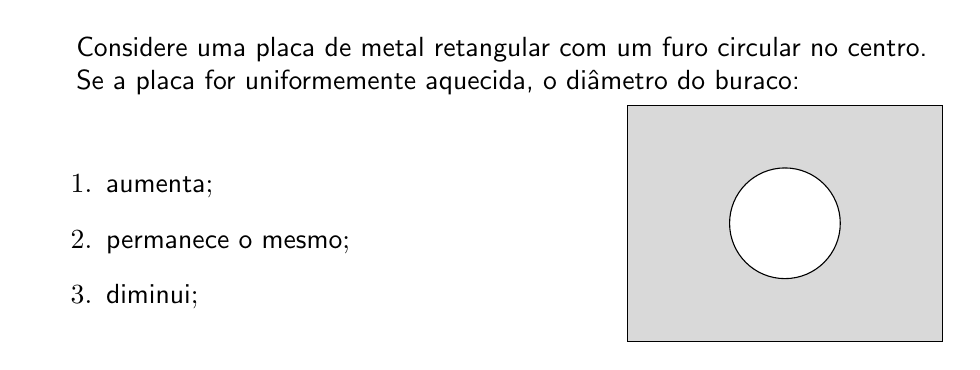
\begin{tikzpicture}[scale=1]
    \label{fig:desenv_ct}
    \node[,text width=11cm] at (0,4) {\textsf{Considere uma placa de metal retangular com um furo circular no centro. Se a
    placa for uniformemente aquecida, o diâmetro do buraco:}};
    \node[,text width=5cm] at (-3.5,2) {
      \begin{enumerate}
        \item \textsf{aumenta};
        \item \textsf{permanece o mesmo};
        \item \textsf{diminui};
      \end{enumerate}
    };
    \draw[fill=gray!30, shift={(1.5cm,.5cm)}](0,0) rectangle (4,3);
    \draw[fill=white, shift={(1.5cm,.5cm)}](2,1.5) circle(20pt);
  \end{tikzpicture}
  \fonte{Adaptado de \cite{Watkins2013}}
\end{figure}

Uma das etapas do IpC na sala de aula é o processo de votação, como mencionado
anteriormente. Existem pelo menos quatro maneiras \cite{Crouch2007} do professor coletar as respostas:

\begin{description}
  \item[Levantar as mãos] a forma mais simples é pedir para os alunos levantarem as mãos para cada alternativa,
  mas dentre as várias limitações desse método temos que os estudantes podem se
  influenciar pela resposta dos outros.
  \item[Cartões colorios] uma segunda alternativa seria o uso de
  cartões coloridos (\textit{flashcards}) que dificultaria os alunos ver a resposta
  dos outros e facilitaria a contagem pelo professor, porém uma limitação desse método,
  assim como o anterior é a dificuldade de alguma forma guardar os resultados.
  \item[Folha de respostas] outra alternativa, no entanto não seria possível ter
  um resultado imediato das respostas.
  \item[Sistemas de resposta em sala de aula] exemplo os \textit{clickers} da \autoref{fig:desenv_clickers}, ou \textit{smartphones},
  e sistemas web possibilitam aos estudantes enviarem imediatamente as respostas ao
  computador do professor, de forma anônima aos colegas de sala e visualizar graficamente
  os resultados.
\end{description}

% 1) a forma mais simples é pedir para os alunos levantarem as mãos para cada alternativa,
% mas dentre as várias limitações desse método temos que os estudantes podem se
% influenciar pela resposta dos outros, 2) uma segunda alternativa seria o uso de
% cartões coloridos (\textit{flashcards}) que dificultaria os alunos ver a resposta
% dos outros e facilitaria a contagem pelo professor, porém uma limitação desse método,
% assim como o anterior é a dificuldade de alguma forma guardar os resultados,
% 3) folha de respostas seria outra alternativa, no entanto não seria possível ter
% um resultado imediato das respostas, 4) já sistemas de resposta em sala de aula como
% os \textit{clickers} da \autoref{fig:desenv_clickers}, ou \textit{smartphones},
% e sistemas web possibilitam aos estudantes enviarem imediatamente as respostas ao
% computador do professor, de forma anônima aos colegas de sala e visualizar graficamente
% os resultados \cite{Crouch2007}.


\begin{figure}
  \begin{centering}
    \caption{\label{fig:desenv_clickers}Exemplo de \textit{clickers}}
    \subfloat[\textit{i>clicker 2}]{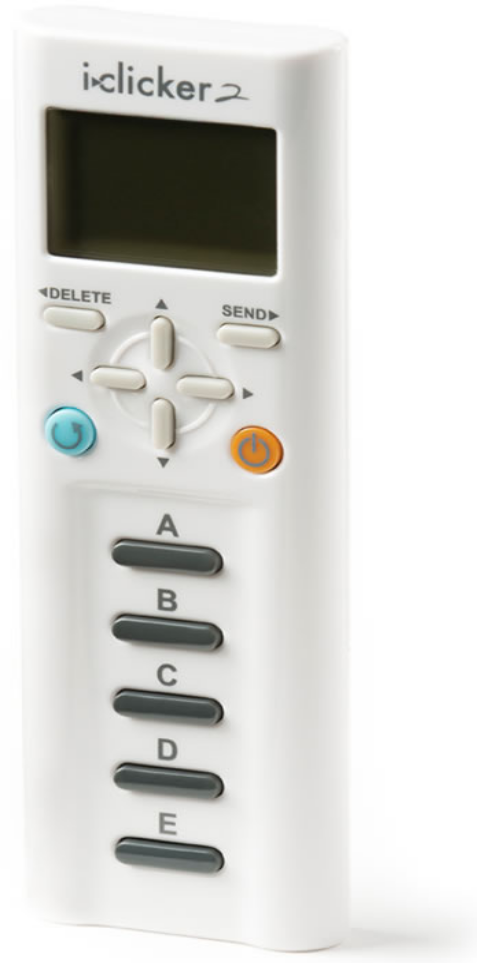
\includegraphics[scale=0.25]{imagens/desenv_iclicker}\label{fig:clickersA}}
    \hspace{.5cm}
    \subfloat[\textit{ResponseCard RF LCD}]{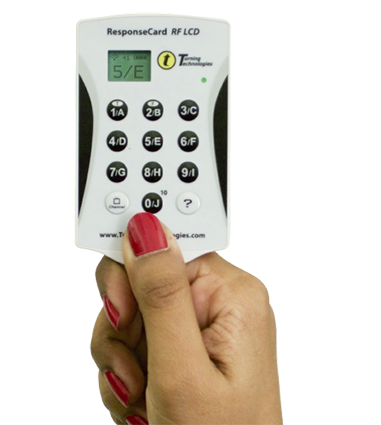
\includegraphics[scale=.4517]{imagens/desenv_turning_clicker}}
    \par
  \end{centering}
  \fonte{(a) \href{http://www1.iclicker.com}{iclicker.com} (b) \href{http://www.turningtechnologies.com}{turningtechnologies.com}}
\end{figure}

No entanto, a implementação do IpC não ocorre apenas na sala de aula. Espera-se
que os alunos façam leituras e atividades antes da aula. Também espera-se do
professor guiar os estudantes nessa etapa, seja indicando ou disponibilizando o
material adequado. O tempo em sala de aula que seria utilizado para apenas transferir
informações para os estudante é utilizado principalmente para discussões, interação
entre os estudantes, tempo para assimilação e para pensar \cite{Mazur2009, Crouch2001}.

\begin{figure}[htbp]
  \centering
  \caption{Diagrama do processo de implementação do método IpC}
  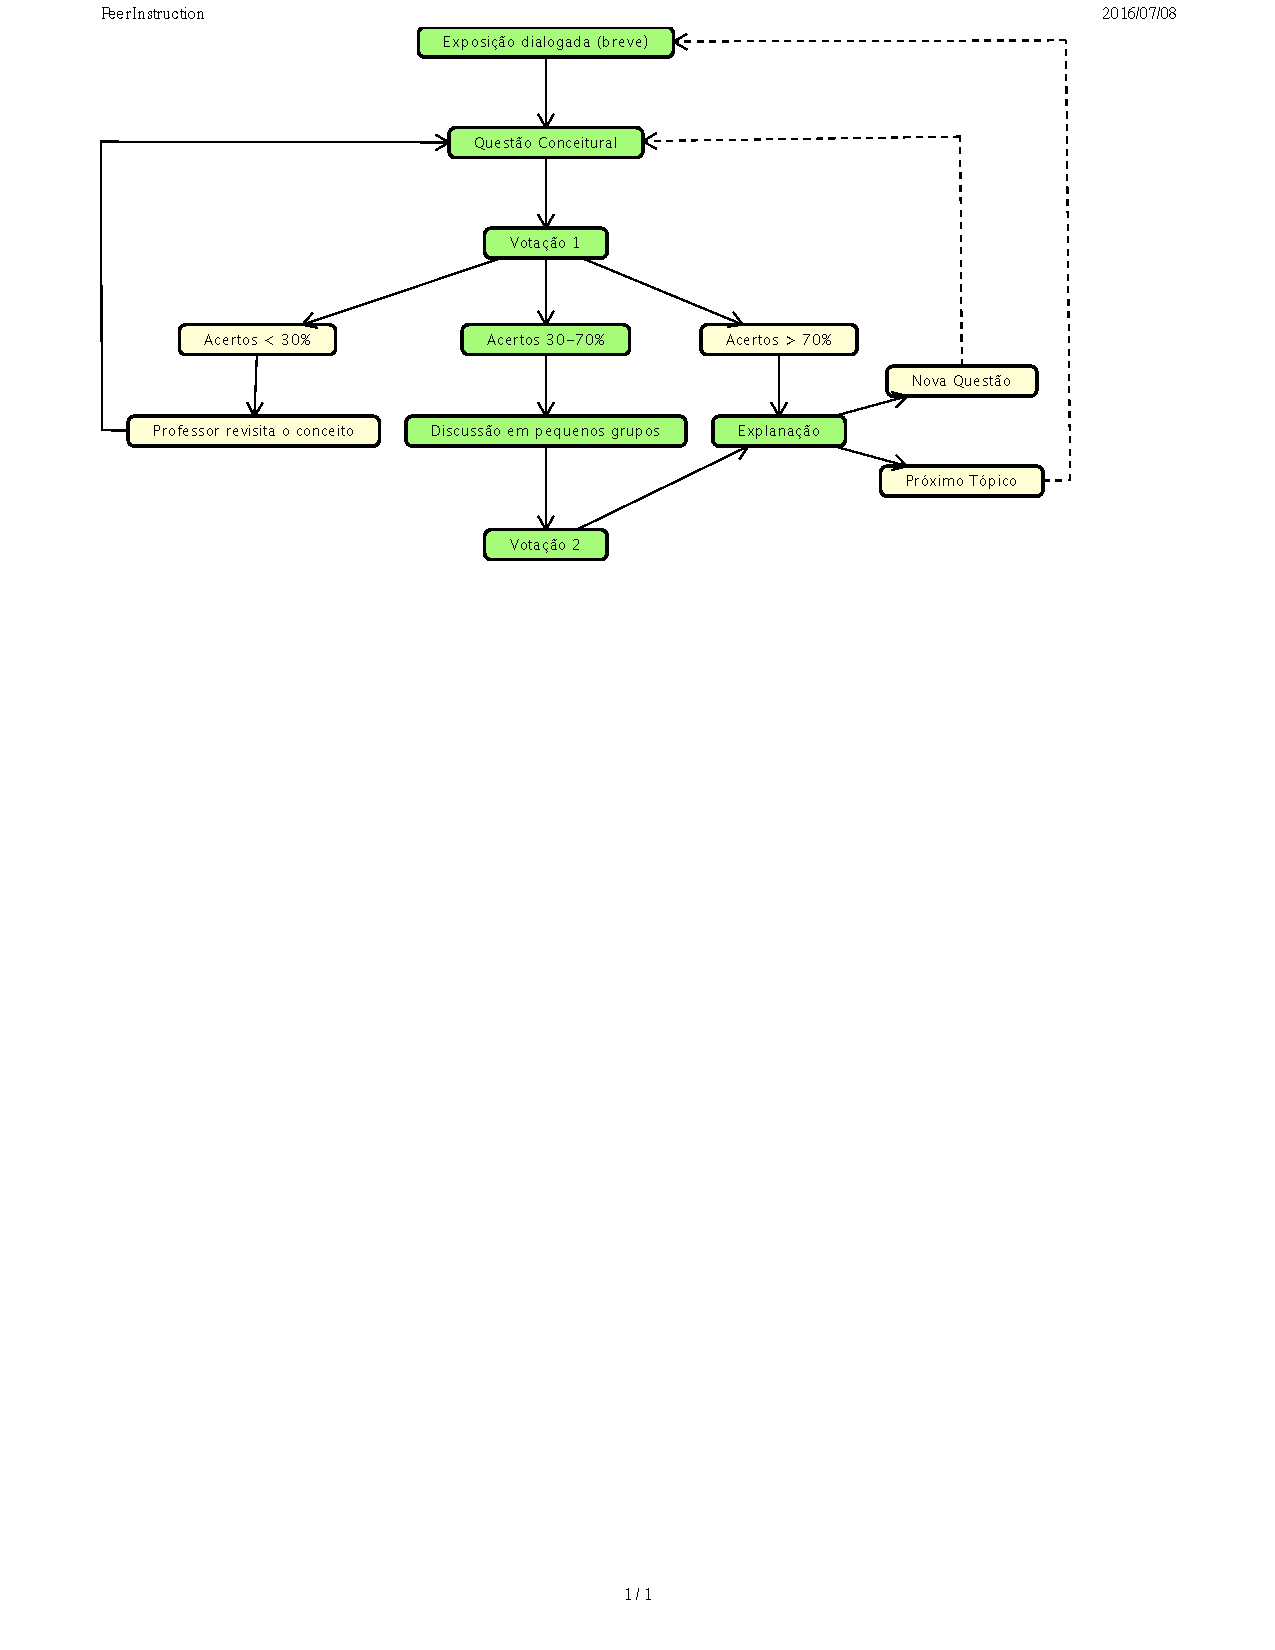
\includegraphics[clip, trim=0cm 18cm 3cm .4cm, width=.85\textwidth]{imagens/peer_instruction}
  \label{fig:desen_fluxograma_ipc}
  \fonte{Adaptado de \cite{Araujo2013}}
\end{figure}


\section{Sistemas de Resposta em Sala de Aula}
\label{section:sistemas_de_resposta}

Sistemas de respostas em sala de aula são tecnologias que permitem ao professor
realizar questionamentos a toda classe e assim obter o resultados das respostas
em tempo real \cite{Kay2009}. Geralmente, as questões são no formato de verdadeiro ou
falso e questões de múltipla escolha. Tais sistemas também podem ser usados para
saber a impressão dos alunos sobre determinado tema \cite{Fies2006}.

Inicialmente introduzido em 1966 na Universidade de Stanford (EUA), os sistemas
de resposta não funcionavam direito, eram difíceis de usar e caros \cite{Kay2009}. Dispositivos
como os da \autoref{fig:desenv_clickers} que usam infravermelho, com preços mais
atrativos, começaram a ser extensivamente usados a partir de 2003 e hoje existe pelo
uma disciplina em cada universidade dos Estados Unidos em que se faz uso de tais sistemas
no processo de ensino e aprendizagem \cite{Abrahamson2014}.

Entretanto, ainda que o custo individual de um aparelho seja atrativo para um
estudante, a realidade da universidade pública brasileira é diferente em relação
a dos Estados Unidos. Assim como não existe obrigatoriedade do aluno comprar um
livro-texto no Brasil, também não existe mecanismo que os faça
comprar \textit{clickers} \cite{GerdKortemeyerEmersonCruz2011}. Dessa forma, os \textit{clickers}
teriam que ser comprados pela universidade, e o custo total não seria tão atrativo.

Veja, por exemplo, a Universidade de São Paulo (USP), em uma tentativa pioneira de
\citeonline{GerdKortemeyerEmersonCruz2011} de oferecer oportunidades para avaliação
formativa usando \textit{clickers} como os da \autoref{fig:clickersA} em duas
turmas de física com 80 alunos cada. Com cada \textit{i>clicker 2}
custando \$43,74 (\textit{vide} \autoref{fig:desenv_preco})
o valor total apenas dos 160 \textit{clickers} seria de
R\$22.116,34\footnote{Considerando o valor do dólar comercial em 12. Ago. 2016
de R\$3,1602. Disponível em: \href{http://www4.bcb.gov.br/pec/taxas/port/ptaxnpesq.asp?id=txcotacao}{http://www4.bcb.gov.br/pec/taxas/port/ptaxnpesq.asp?id=txcotacao}},
necessitando ainda do aparelho que recebe as respostas, software que é instalado
no computador do professor, treinamento e suporte, ou seja, o valor final pode ser
ainda maior. A propósito, esse é uma das principais barreiras na adoção dessa
ferramenta no processo de ensino, que ainda tem a resistência de alguns professores
em usar novas tecnologias como ferramentas de ensino \cite{Blasco-Arcas2013, GerdKortemeyerEmersonCruz2011, Kay2009}.

\begin{figure}[!t]
  \centering
  \caption{Preço do \textit{i>clicker 2}}
  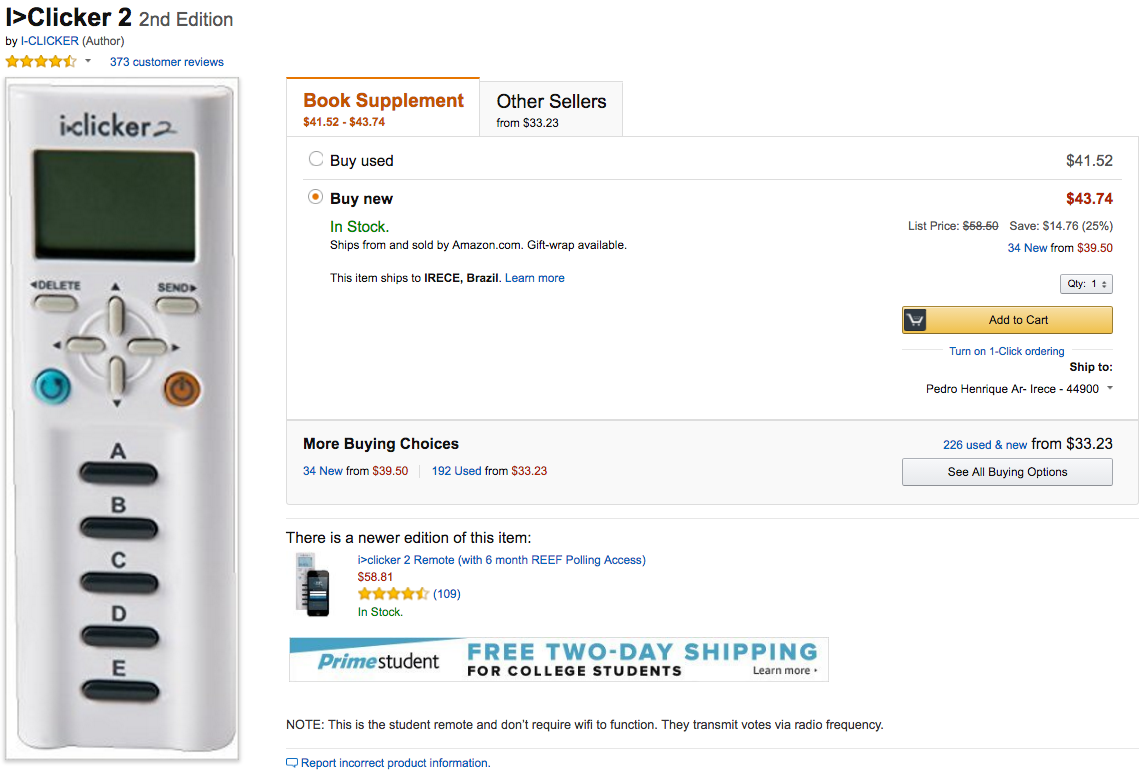
\includegraphics[width=.75\textwidth]{imagens/desenv_preco}
  \fonte{\href{https://goo.gl/q4nBdg}{amazon.com} pesquisando \textit{i>clicker 2}. Acesso em 12. Ago. 2016}
  \label{fig:desenv_preco}
\end{figure}

Todavia, uma maneira de tornar tal tecnologia mais acessível é usar os próprios
celulares dos estudantes como {\clickers} \cite{Stowell2015, Morrell2015, Araujo2013}.
Além de mais acessível, usando os próprios celulares, os estudantes podem
ver as questões e os resultados da classe nos próprios aparelhos. Para o professor,
uma variedade maior de questões podem ser exploradas, como uma  questão aberta \cite{Stowell2015}.

Saliente-se ainda que, embora possa haver um pequeno aumento no número de questões
sem respostas, as respostas dos estudantes são comparáveis quando se usa
\textit{clickers} \cite{Morrell2015, Stowell2015}.

Ainda que o uso do celular como {\clicker} possa aumentar o nível de
distrações, são muitos os benefícios de usar essa abordagem, no entanto,
é preciso estar atento aos pequenos casos de estudantes que não têm a tecnologia
adequada, ou que não queiram usar os seus dispositivos \cite{Morrell2015, Stowell2015}.

\subsection*{\textit{Smartphones} no Brasil}

É importante aqui destacar o uso dos dispositivos que podem permitir essa abordagem
na realidade brasileira. Hoje existem 1,2 dispositivos portáteis
(\textit{smartphones} e \textit{tablets}) por habitante e uma projeção para o próximo
biênio 2017/2018 de 2 dispositivos
(desktops, \textit{notebooks}, \textit{tablets} e \textit{smartphones}) por habitante \cite[p. 8]{Meirelles2016}.
Acrescenta-se também que já em 2014 mais de 93\% dos estudantes da rede privada de
ensino e quase 67\% dos da rede pública possuem \textit{smartphones}, em que a
proporção de pessoas é maior na rede pública \cite[p. 55]{IBGE2016}. Também cabe
ressaltar que o celular já é o principal meio para acessar a Internet nos domicílios
brasileiros \cite[p. 41]{IBGE2016}.

\subsection*{Alternativas Disponíveis}
\label{subp:alternativas_disponiveis}

Cabe a este respeito apresentar algumas soluções disponíveis que permitem usar o celular como
{\clicker}.

Em um estudo para desenvolver uma estratégia de ensino utilizando
{\clickers} como recurso didático \citeonline{Mattos2015}, utilizou o
\href{https://www.polleverywhere.com/}{\textit{Poll Everywhere}} que foi
escolhido principalmente por ser compatível com as principais plataformas
móveis (Android, iOS e Windows Phone). O
\href{https://www.polleverywhere.com/}{\textit{Poll Everywhere}} oferece uma
versão gratuita com no máximo 40 respostas por votação com algumas limitações.
Na versão paga, o estudante pode pagar \$14/ano ou o professor pode pagar
\$349/semestre (vide \autoref{fig:polleverywhere}).

Outra solução é o \href{http://www.socrative.com/}{\textit{Socrative}},
que também é compatível com todas as plataformas, e na sua versão gratuita
permite até 50 alunos por votação, questões de múltipla escolha, de verdadeira e falso,
resposta curta, \textit{quizzes}, etc \cite{socrative2016}. Alguns relatos do uso do
\href{http://www.socrative.com/}{\textit{Socrative}} em sala de aula para promover
a interatividade são encontrados em \cite{Kaya2016, Trindade2014}.
Uma opção interessante do \href{http://www.socrative.com/}{\textit{Socrative}}
é o \textit{Exit Ticket}, em que ao final da aula os estudantes respondem
a três perguntas. A primera funciona como uma auto-avaliação, perguntando
o quanto o estudante entendeu da aula, já as outras duas como identificação, que são o
nome do aluno e uma pergunta que o professor coloca no quadro, ou seja, teoricamente,
apenas os alunos presentes vão ser capazes de responder corretamente, servindo
então como um controle de frequência. Na versão paga o professor pode pagar \$49,99/ano (vide \autoref{fig:socrative}).

Por último, o aplicativo \href{http://www.tophat.com/}{\textit{TopHat}}, que parece
ser usado diariamente por mais 500 instituições de ensino pelo mundo \cite{tophat2016}.
Para o professor, \href{http://www.tophat.com/}{\textit{TopHat}} permite incorporar
uma variedade de questões, também uma revisão interativa da aula e para provas
\cite{Neilson2016}. A inscrição mais popular no  \href{http://www.tophat.com/}{\textit{TopHat}}
são de \$36/ano (vide \autoref{fig:tophat})

\begin{figure}
  \centering
  \caption{Preço de algumas sistemas de resposta}
  \subfloat[Disponível em: \href{https://www.polleverywhere.com/plans/higher-ed}{polleverywhere.com/plans/higher-ed}: em 16 ago. 2016]{
    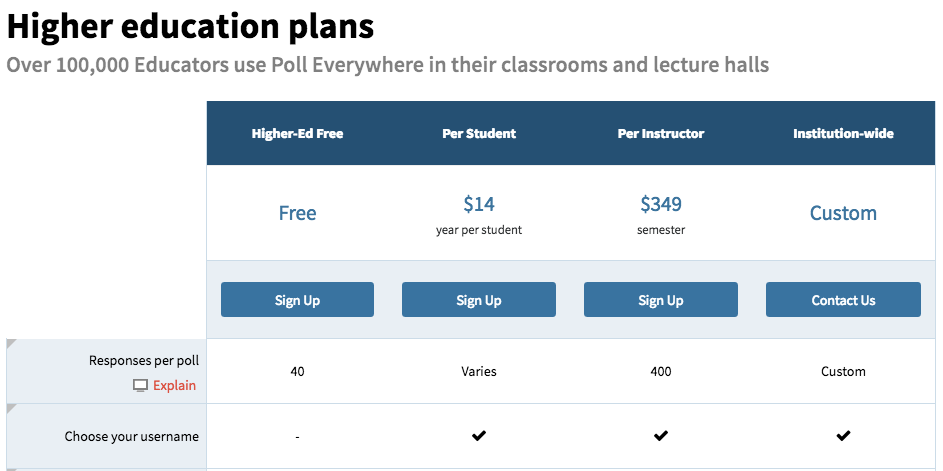
\includegraphics[scale=0.35]{imagens/polleverywhere2}
    \label{fig:polleverywhere}
  }

  \subfloat[Disponível em: \href{http://www.socrative.com/pricing.php}{socrative.com/pricing}: em 16 ago. 2016]{
    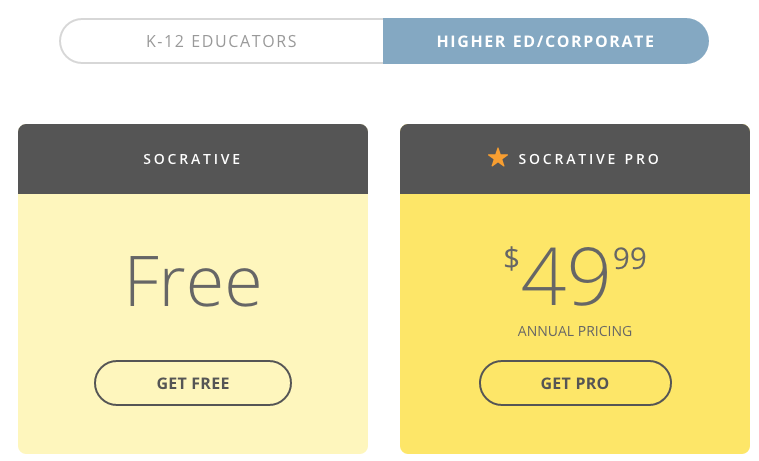
\includegraphics[scale=0.35]{imagens/socrative}
    \label{fig:socrative}
  }

  \subfloat[Disponível em: \href{https://tophat.com/pricing/}{tophat.com/pricing} em: 16 ago. 2016]{
    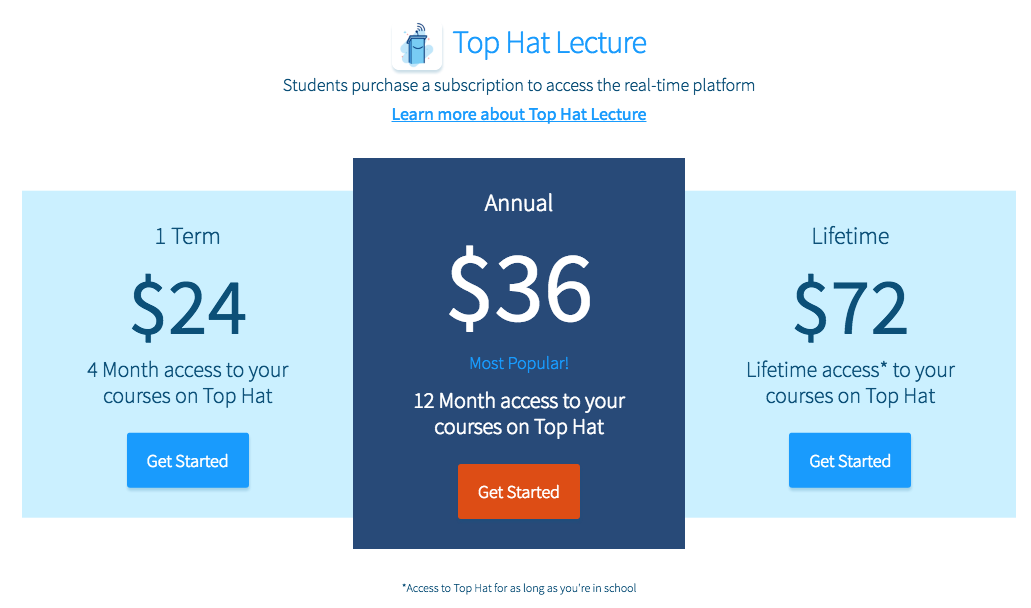
\includegraphics[scale=0.35]{imagens/tophat}
    \label{fig:tophat}
  }
\end{figure}

\subsection{Uso dos Sistemas de Resposta em Sala de Aula}

Lorem ipsum dolor sit amet, consectetur adipisicing elit, sed do eiusmod tempor incididunt ut labore et dolore magna aliqua. Ut enim ad minim veniam, quis nostrud exercitation ullamco laboris nisi ut aliquip ex ea commodo consequat. Duis aute irure dolor in reprehenderit in voluptate velit esse cillum dolore eu fugiat nulla pariatur. Excepteur sint occaecat cupidatat non proident, sunt in culpa qui officia deserunt mollit anim id est laborum.

% Com efeito, a tecnologia apresenta-se como meio, como instrumento para colaborar no desenvolvimento do processo de aprendizagem. A tecnologia reveste-se de um valor relativo e dependente desse processo. Ela tem sua importância apenas como um instrumento significativo para favorecer a aprendizagem de alguém. Não é a tecnologia que vai resolver ou solucionar o problema educacional do Brasil. Poderá colaborar, no entanto, se for usada adequadamente, para o desenvolvimento educacional de nossos estudantes.

\clearpage
\section{Engenharia de Software}

Engenharia de Software pode ser definida como:
\begin{citacao}[english]
1. the systematic application of scientific and technological knowledge, methods, and experience to the design,
implementation, testing, and documentation of software [...]  2. the application
of a systematic, disciplined, quantifiable approach to the development, operation,
and maintenance of software; that is, the application of engineering to software \cite{IEEE2010}.
\end{citacao}

A engenharia de software deve ter foco na qualidade, que apoia as outras camadas
dessa tecnologia, que são as camadas de processo, métodos e ferramentas \autoref{fig:desen_engsoft}.
A camada de processo define um conjunto de atividades ou um arcabouço que tem
como finalidade garantir a efetiva utilização da tecnologia engenharia de software, que então
leva à produção de um software. Os detalhes de como fazer o software pertencem
a camada de métodos. Os métodos da enghenharia de software incluem tarefas de planejamento
e estimativa de software, análise de requisitos, modelagem de projeto, codificação,
testes e manutenção. As ferramentas de engenharia de software auxiliam as camadas de
processo e métodos, com ferramentas automatizadas, que por sua vez, quando integradas,
é estabelecido um suporte ao desenvolvimento de software chamado CASE -
\textit{Computer Aided Software Engineering} \cite{Pressman2009, Sommerville2006}.

\begin{figure}[b]
  \centering
  \caption{Engenharia de Software - uma tecnologia em camadas}
  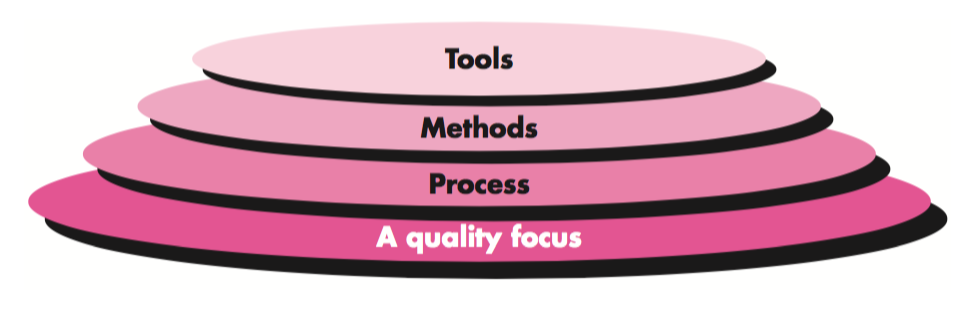
\includegraphics[scale=0.3]{imagens/desenv_engsoft2}
  \label{fig:desen_engsoft}
  \fonte{\cite{Pressman2009}}
\end{figure}

Entre o conjunto de atividades definidas pela camada de processo, quatro são
fundamentais, a saber, especificação de software, projeto e implementação de
software, validação de software e evolução de software. Especificação de software
ou engenharia de requisitos é uma fase importante e crítica do processo de engenharia
de software. Importante porque é uma análise de requisitos bem feita que possibilitará
atendar as demandas dos usuários. Crítica porque um sistema mal especificado, pode até ser
bem projetado e construído, mas não vai atender as necessidades dos usuários.
Em seguida, na fase de projeto e implementação os requisitos são projetados e programados,
tendo como resultado um sistema executável. Depois, o software deve ser verificado
para mostrar que atende às demandas dos usuários (validação do software). Finalmente,
na fase de evolução de software, o software é modificado devido às mudanças
de requisitos e às necessidades dos usuários.

